%%
%% Framesoc User Guide
%%

\documentclass[twoside]{article}
\usepackage[a4paper]{geometry}
\usepackage[utf8]{inputenc}
\usepackage[T1]{fontenc}
\usepackage{RR}
\usepackage{epsfig}
\usepackage[frenchb]{babel}
\usepackage{cite}
\usepackage{float}
\usepackage{graphicx}
\usepackage{subcaption}
\usepackage{textcomp}
\usepackage[hidelinks]{hyperref} % hide link squares
\usepackage{listings}
%%
%% date
\RRdate{December 2014}
%%
%% If version 2
%% \RRversion{2}
%% version 2 date
%% \RRdater{November 2008}
%%
\RRauthor{
Generoso Pagano \thanks{INRIA, generoso.pagano@inria.fr}
}
%% On each even page
\authorhead{Framesoc User Guide [DRAFT]}
%% French title
\RRtitle{Framesoc User Guide [DRAFT]}
%% English title
\RRetitle{Framesoc User Guide [DRAFT]}
%%
\titlehead{Framesoc User Guide [DRAFT]}
%%
\RRprojet{MESCAL}
%%
\URRhoneAlpes 
%%
\RCGrenoble 
%%
\abstract{This guide describes the Framesoc workbench, which is the desktop user environment provided by Framesoc infrastructure. The document targets the end-users.}

%%=====================================================================
%%=====================================================================
\begin{document}

\begin{sloppypar} %% avoid long words exceeding margins
%%=====================================================================
%%=====================================================================

\shorthandoff{:} %% Remove the space before the colon
\interfootnotelinepenalty=10000 %% allow long footnotes

%%=====================================================================
%% Custom commands
\newcommand{\parag}[1]{\paragraph{#1}\mbox{}\\}
\newcommand{\subparag}[1]{\subparagraph{#1}\mbox{}\\}
\newcommand{\subsubparag}[1]{\subparagraph{#1}}
\newcommand{\num}[1]{\textcolor{red}{#1}}

%% 
%% Itemize
\renewcommand{\labelitemi}{$\bullet$}
\renewcommand{\labelitemii}{$\circ$}
%%=====================================================================

%%
\makeRT 
%%

%%=====================================================================
\renewcommand{\contentsname}{Table of contents}
\tableofcontents
\newpage
%%=====================================================================
%=====================================================================
\section{Introduction}
\label{sec:introduction}

%=====================================================================

Framesoc, the SoC-Trace project~\cite{SoC-TRACE} trace management infrastructure, is composed by three main layers, as shown in Figure~\ref{fig:architecture}.

\begin{figure}[h]
  \centering
    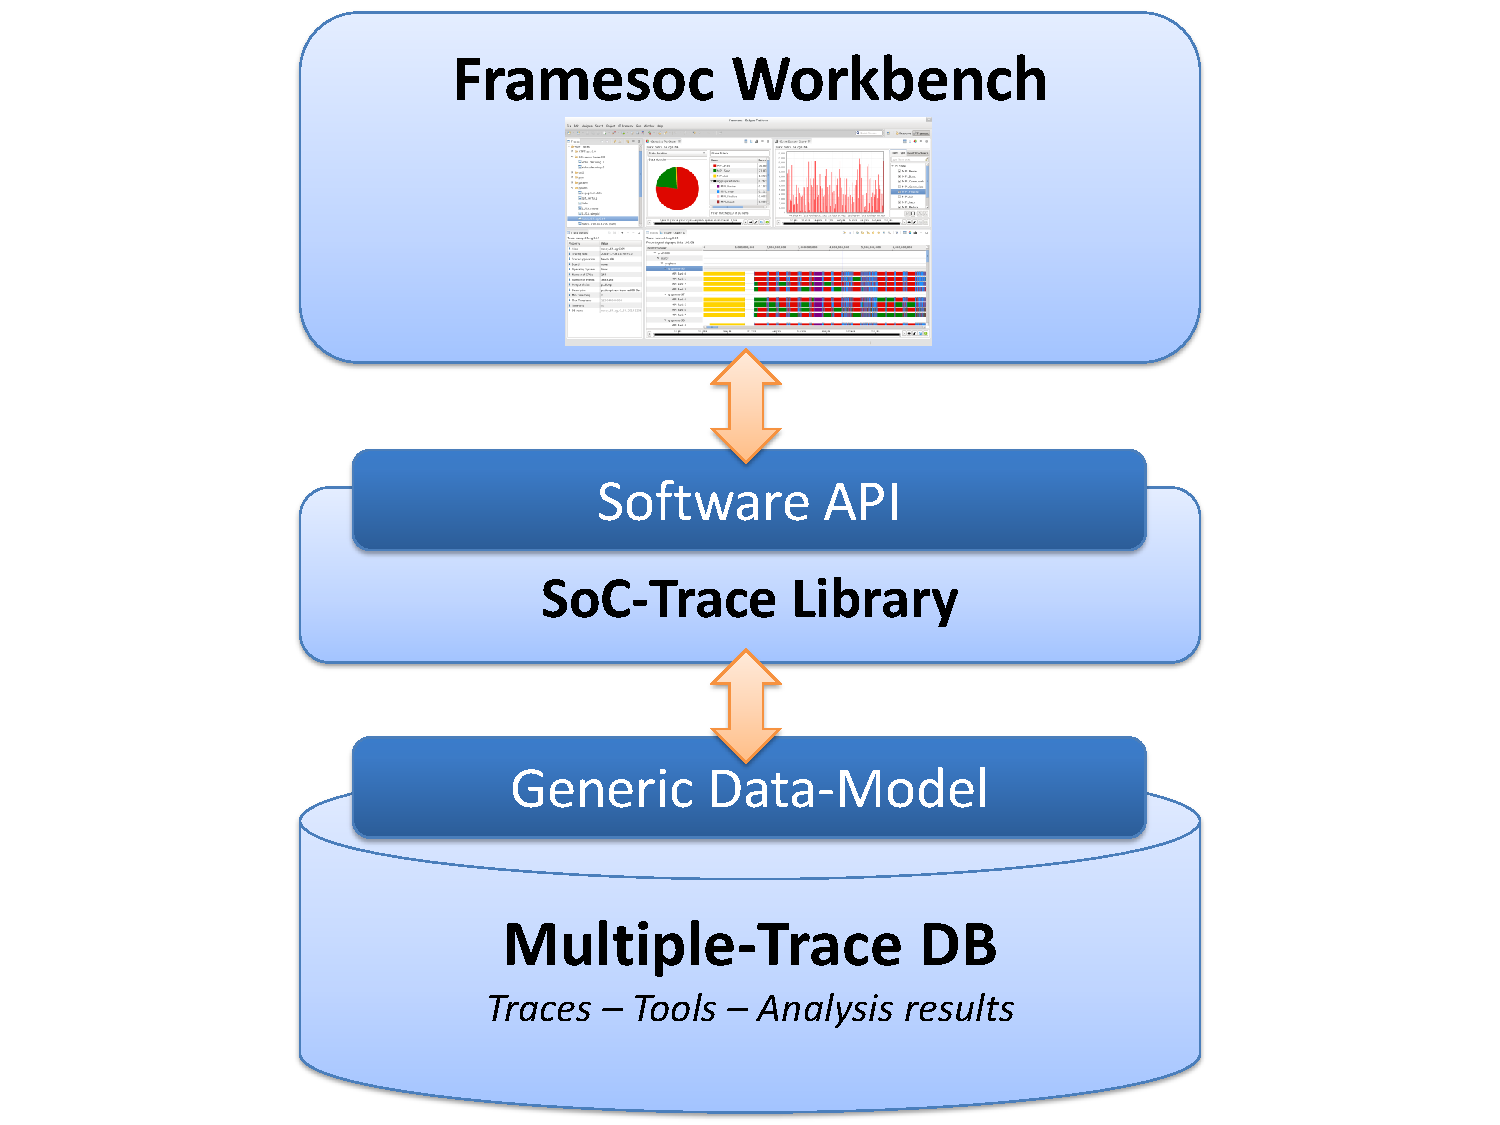
\includegraphics[width=0.7\textwidth]{images/framesoc_architecture.pdf}
  \caption{Framesoc Architecture}
  \label{fig:architecture}
\end{figure}

At the lowest level, there is a Multiple-Trace database, which stores all the data concerning traces, analysis tools and the analysis result produced by thees tools, using a generic data-model.
Above this layer, the SoC-Trace library provides a software API to facilitate the interaction with the data-model and help the implementation of trace tools.
On top of this software library, Framesoc provides a graphical user environment, facilitating trace management, basic trace analysis and tool management.

This guide describes Framesoc from the user perspective (i.e., Framesoc graphical user environment). 
More information about the lowest layers of Framesoc infrastructure can be found in the technical report RT-427~\cite{pagano:hal} and the research report RR-LIG-046~\cite{rrlig46}.

\newpage

%=====================================================================
\section{Installation and Setup}
\label{sec:installation}
%=====================================================================

Framesoc is an application built on top of the Eclipse framework. Therefore, the easyest way to install Framesoc is to use its Eclipse update site, as explained in the online wiki page: \url{https://github.com/soctrace-inria/framesoc/wiki/Install-and-setup-a-standalone-version-of-Framesoc-using-the-update-site}.

%=====================================================================
\section{Framesoc Perspective}
\label{sec:perspective}
%=====================================================================

\begin{figure}[h!]
  \centering
    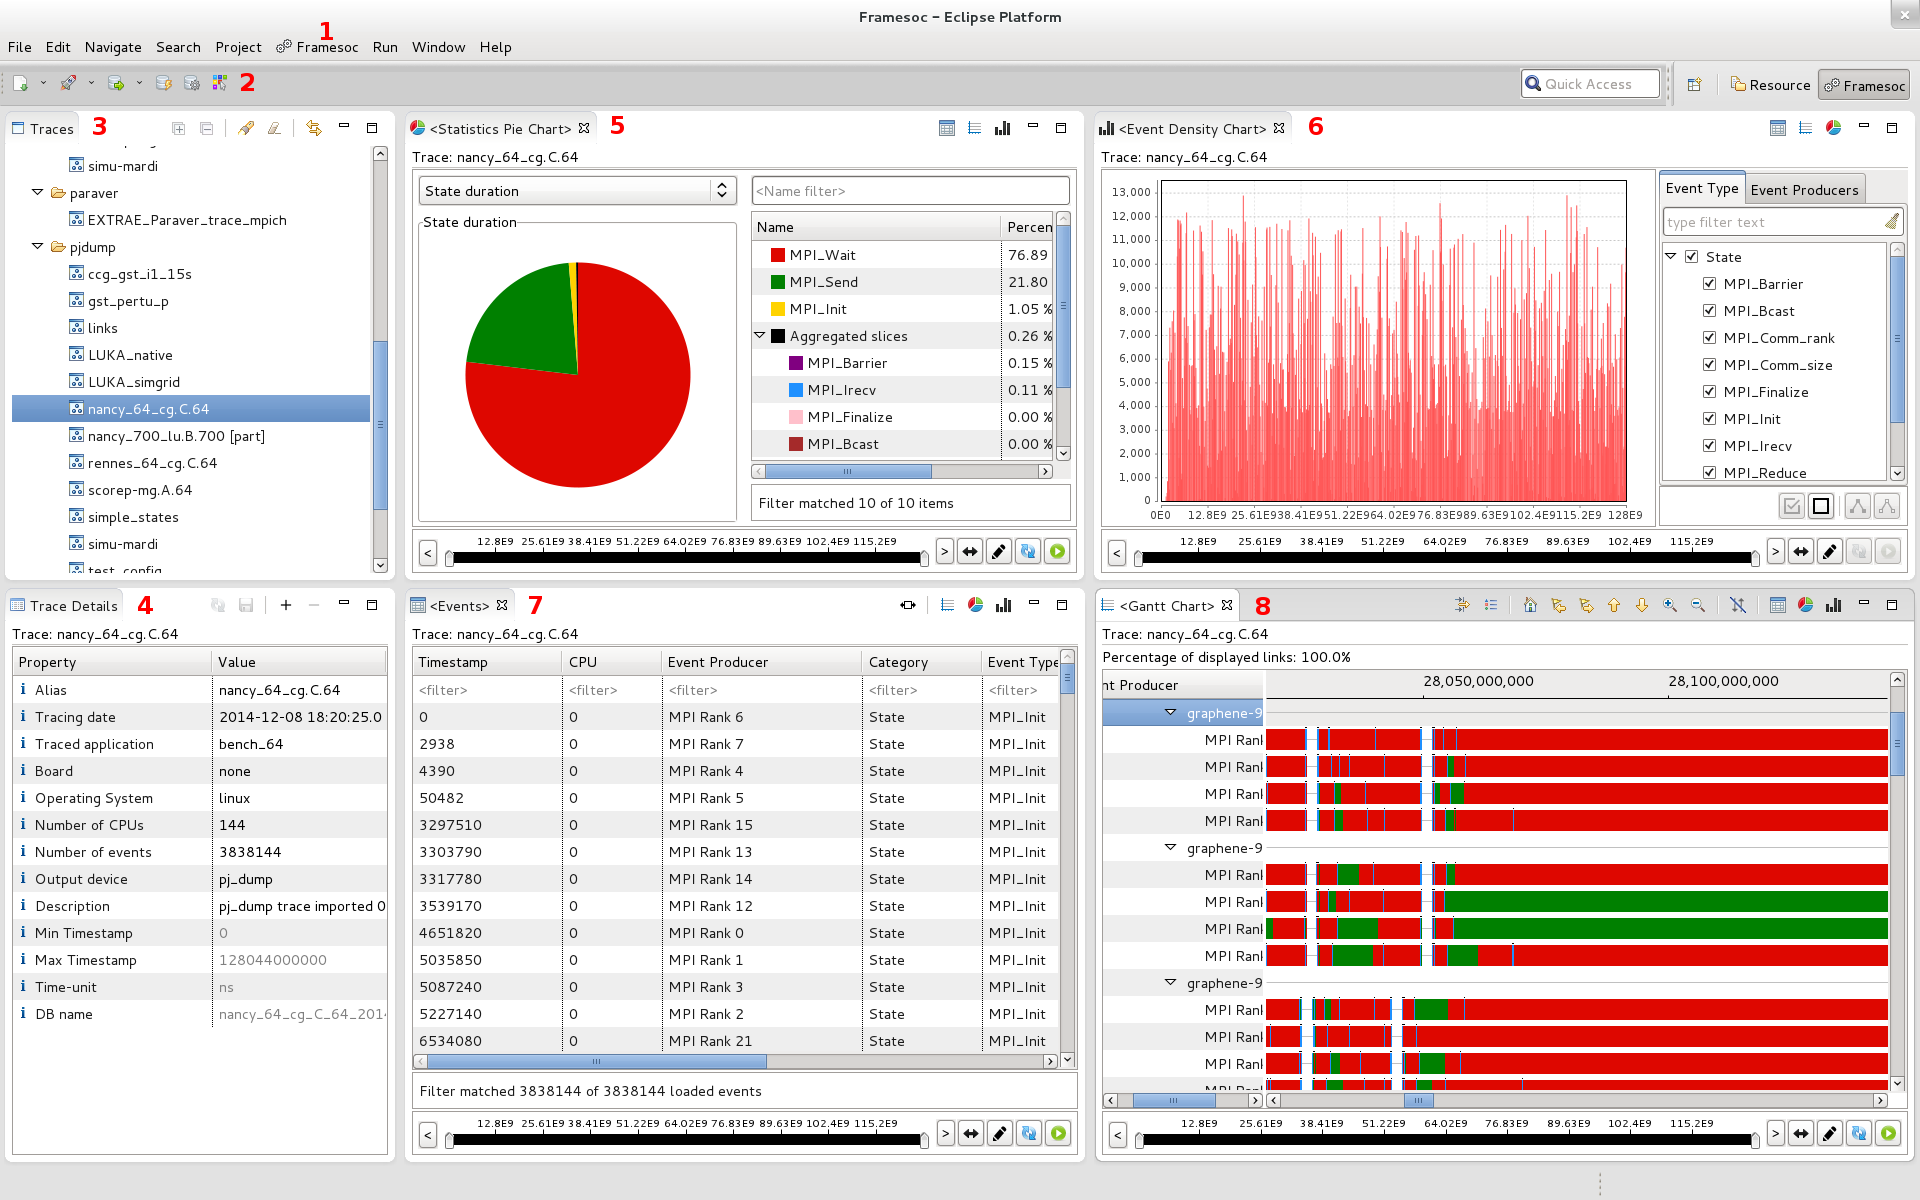
\includegraphics[width=1.0\textwidth]{images/perspective_numbers.png}
  \caption{Framesoc Eclipse Perspective}
  \label{fig:all_perspective}
\end{figure}

Framesoc provides an Eclipse perspective\footnote{Within an Eclipse application, a perspective defines an initial set and layout of views, menu and toolbars. The Framesoc Eclipse perspective can be activated by selecting it from the \textbf{Window > Open Perspective > Other... > Framesoc} menu.} for trace management and analysis.
The Framesoc perspective (Figure~\ref{fig:all_perspective}) contains the following elements:
\begin{itemize}
 \item A Framesoc menu (\num{1}).
 \item A toolbar (\num{2}).
 \item A set of views for trace management and analysis. We find on the left the two \emph{management views}: a trace browser (\num{3}) and a trace metadata viewer/editor (\num{4}). On the right, there are four \emph{analysis views}: a statistics pie chart (\num{5}), an event density chart (\num{6}), an event table (\num{7}), and a Gantt chart (\num{8}). 
\end{itemize}

The management views (trace browser and metadata viewer/editor) refer to the whole system and are typically the entry point for trace analysis.
For this reason, they cannot be closed and there can be only a single instance of each of them.
On the contrary, all the analysis views refer to a single trace, so they can be opened and closed as needed. 
For each trace, there can be an instance of each type of analysis view. 
The maximum number of open instances for a given type of analysis view is configurable (Appendix~\ref{app:conf}).
When a trace is selected in the trace browser, the corresponding metadata are shown in the metadata viewer and all the analysis views referring to that trace (if any) are highlighted. Namely, the view name is surrounded by \emph{<} and \emph{>}. 
In the example shown in Figure~\ref{fig:all_perspective}, all analysis views refer to the selected trace \texttt{nancy\_64\_cg.C.64}).
On the other hand, when an analysis view is given focus, the trace shown in that view becomes the selected trace in the trace browser, so the metadata viewer is updated accordingly and all the analysis views are consistently highlighted or unhighlighted. 

The following sections describe in detail Framesoc management and analysis views, as well as the functionalities accessible via Framesoc menu and toolbar.

%=====================================================================
\section{Management Views}
\label{sec:management}
%=====================================================================

%------------------------------------------------------------------
\subsection{Trace Browser}
\label{subsec:explorer}

\begin{figure}[h!]
  \centering
    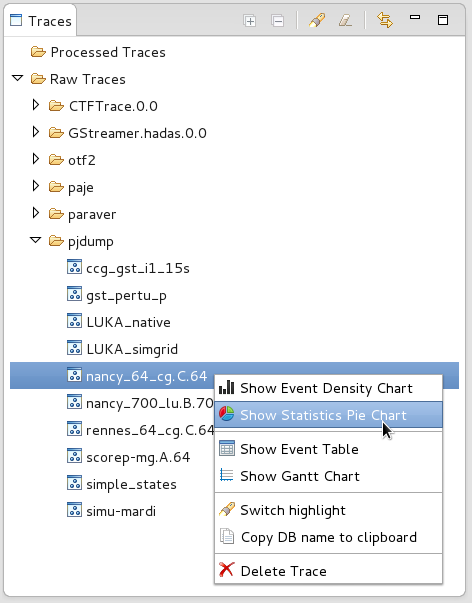
\includegraphics[width=0.5\textwidth]{images/trace_browser_popup.png}
  \caption{Traces view}
  \label{fig:popup_explorer}
\end{figure}

The \emph{Traces} view (Figure~\ref{fig:popup_explorer}) is the Framesoc perspective trace browser.
Traces are presented in a tree viewer with a two-level hierarchy. 
The first level distinguishes processed traces from raw traces~\footnote{As described in the technical report RT-427~\cite{pagano:hal}, a processed trace is a trace created by an analysis tool as the result of an analysis on another trace.}. 
Then, in each of these two categories, traces are grouped by type. 
The type may relate to the trace format or to the tool that created the trace. 
The viewer presents a trace alias for each trace.

Double-clicking on a trace opens the Event Density Chart for that trace (Subsection~\ref{subsec:histogram}).
Right-clicking on a single trace opens a context menu that gives access to the following functionalities:
\begin{itemize}
 \item \emph{Show Event Density Chart}: open the density chart view for this trace (see Subsection~\ref{subsec:histogram}).
 \item \emph{Show Statistics Pie Chart}: open the pie chart view for this trace (see Subsection~\ref{subsec:pie}).
 \item \emph{Show Event Table}: open the event table view for this trace (see Subsection~\ref{subsec:table}).
 \item \emph{Show Gantt Chart}: open the Gantt chart view for this trace (see Subsection~\ref{subsec:gantt}).
 \item \emph{Switch highlight}: switch the highlight state of the trace in the browser (see Figure~\ref{fig:highlight}). A trace being highlighted in the browser is shown in bold.
 \item \emph{Copy DB name to clipboard}: copy to the clipboard the name of the database containing the trace raw data.
 \item \emph{Delete Trace}: delete the trace from the system.
\end{itemize}
If more traces are selected, only the \emph{Switch highlight} and \emph{Delete Trace} entries are displayed in this context menu.
Note that if one or more traces are deleted, an update notification is sent to the other views.
This allows a view to do the necessary actions if the trace it displays has been deleted.

The view toolbar contains the following buttons: a couple of buttons to expand (\num{1}) and collapse (\num{2}) the trace hierarchy, a button to launch the \emph{Trace Filter Dialog} (\num{3}, see Subsection~\ref{subsubsec:trace_filter}), a button to clean the highlight state of all traces (\num{4}, see Subsection~\ref{subsubsec:trace_filter}) and a button to manually resynchronize the displayed traces with the information contained in the Framesoc System DB\footnote{See the technical report RT-427~\cite{pagano:hal} for further details on the database architecture.} (\num{5}).

\subsubsection{Trace Filter}
\label{subsubsec:trace_filter}

Pressing the button indicated as \num{3} in Figure~\ref{fig:popup_explorer}, the \emph{Trace Filter Dialog} is opened (Figure~\ref{fig:trace_filter_dialog}).

\begin{figure}[h!]
  \centering
    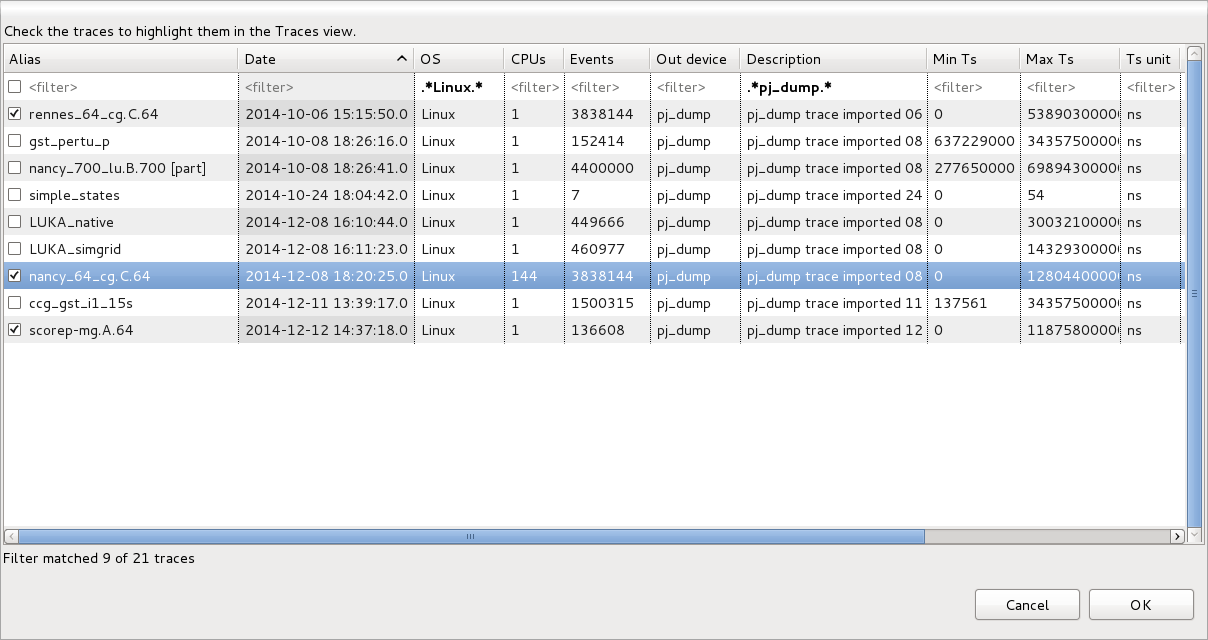
\includegraphics[width=0.9\textwidth]{images/trace_table_filter.png}
  \caption{Trace Filter Dialog}
  \label{fig:trace_filter_dialog}
\end{figure}

This dialog displays a table containing all the traces imported in the system. Each column of this table corresponds to a particular trace metadata. Clicking on the header of each column, it is possible to sort the table rows according to the column content. The first row of the table has editable fields, allowing for filtering on the corresponding column content. Filtering can be done using regular expression. In the example shown in Figure~\ref{fig:trace_filter_dialog}, we filtered all the traces produced on ``Linux'', containing the string ``pj\_dump'' in the description.

The first column of each row has a checkbox, allowing to select/deselect the corresponding trace. The checkbox in the first row (filter row) select/deselect all shown traces.
When pressing \emph{OK}, all selected traces are highlighted (shown in bold) in the trace browser (Figure~\ref{fig:highlight}). This allows the analyst to immediately spot interesting traces in the browser.

\begin{figure}[h!]
  \centering
    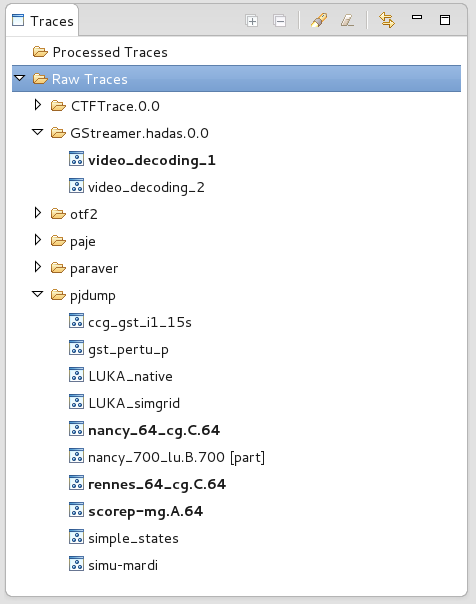
\includegraphics[width=0.5\textwidth]{images/trace_browser_highlight.png}
  \caption{Highlighted traces in Traces view}
  \label{fig:highlight}
\end{figure}

%------------------------------------------------------------------
\subsection{Trace Metadata Viewer/Editor}
\label{subsec:metadata}

\begin{figure}[h!]
  \centering
    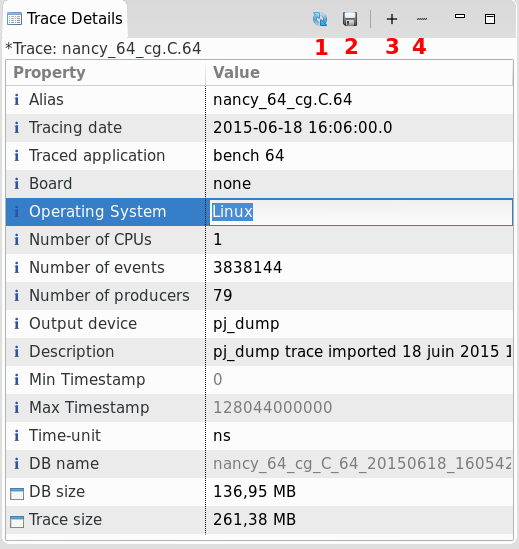
\includegraphics[width=0.5\textwidth]{images/metadata_editing.png}
  \caption{Trace Details view}
  \label{fig:metadata_editing}
\end{figure}

The \emph{Trace Details} view (Figure~\ref{fig:metadata_editing} is the Framesoc perspective trace metadata viewer and editor.
When a trace is selected in the \emph{Traces} view, the trace metadata are displayed in a table viewer containing two columns: the property name and the property value.
If more than one trace is selected in the \emph{Traces} view, only the properties having the same name and the same values are shown.
The different properties are grouped in two different categories: predefined properties (displayed first) and custom properties (displayed last). 
Those categories are identified by two different icons.
The \emph{Value} column is normally editable, with the exception of some properties that are read only.
In order to edit an editable property value, the user simply has to click the value and modify it (as shown in Figure~\ref{fig:metadata_editing} for the \emph{OS} property).
When one or more values have been modified, a star (\emph{*}) is displayed before the trace alias, on top of the table, and the two view toolbar buttons \num{1} and \num{2} are enabled. 
The \emph{Reset changes} button (\num{1}) restores all non-saved edited properties to their previous value.
The \emph{Save changes} button (\num{2}) stores the changes.
%% TODO the notification must be done for any metadata change!!! cfr. issue #106
If the \emph{Alias} predefined property of a trace is persistently modified, other views are notified in order to take the necessary actions (e.g., update their label for the trace).

The other two buttons in the toolbar (\num{3} and \num{4}) allows for adding and removing custom trace metadata to the currently selected traces. Pressing the button indicated with \num{3} in Figure~\ref{fig:metadata_editing}, a dialog to add a new property is shown (Figure~\ref{fig:new_metadata}).

\begin{figure}[h!]
  \centering
    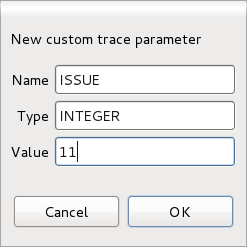
\includegraphics[width=0.3\textwidth]{images/new_metadata.png}
  \caption{Dialog to add a new custom property as trace metadata}
  \label{fig:new_metadata}
\end{figure}

In the example shown in Figure~\ref{fig:new_metadata}, after pressing \emph{OK}, a new trace property \texttt{ISSUE} of type \texttt{INTEGER} and value \texttt{11} is added to the selected trace. The trace metadata will therefore look as shown in Figure~\ref{fig:metadata_remove}. In this figure it is possible to see that, when selecting a custom property, the \emph{Remove property} button (indicated as \num{4} in Figure~\ref{fig:metadata_editing}, where it is disabled) is enabled and can be used to remove the selected custom property.

\begin{figure}[h!]
  \centering
    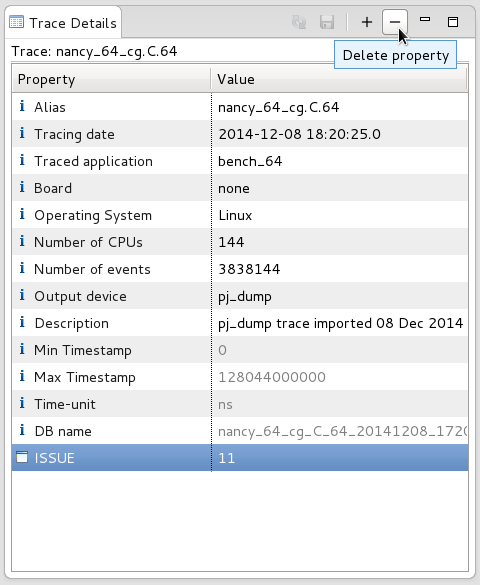
\includegraphics[width=0.5\textwidth]{images/metadata_remove.png}
  \caption{Trace Details view after adding a custom property (ISSUE)}
  \label{fig:metadata_remove}
\end{figure}

Note that if more than one trace is selected in the \emph{Traces} view, it is still possible to edit, add or remove properties.

%=====================================================================
\section{Analysis Views}
\label{sec:analysis}
%=====================================================================

%------------------------------------------------------------------
\subsection{Statistics Pie Chart}
\label{subsec:pie}

%%% TODO

\begin{figure}[h!]
  \centering
    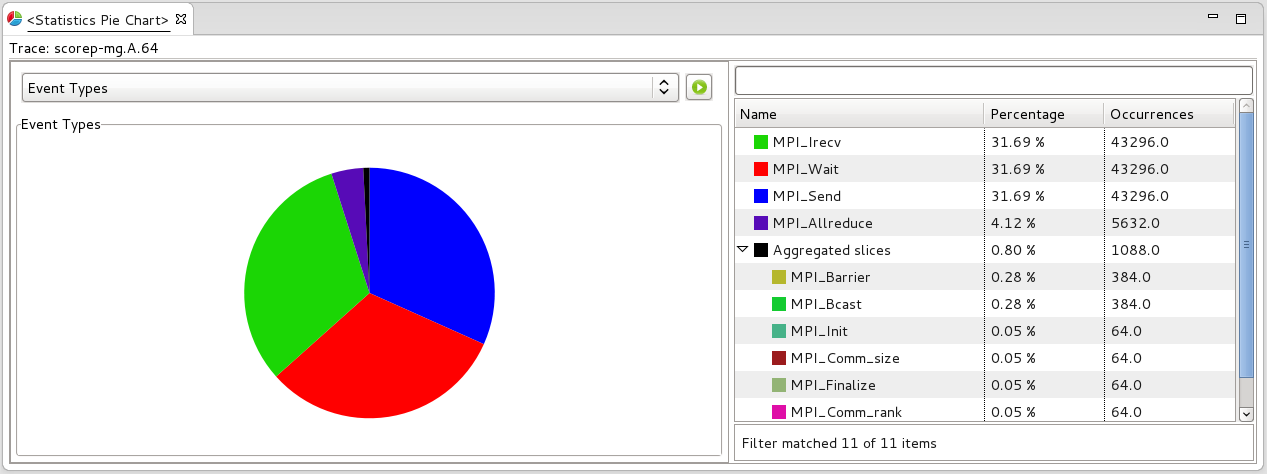
\includegraphics[width=1.0\textwidth]{images/pie_chart.png}
  \caption{Statistics Pie Chart view}
  \label{fig:pie_chart}
\end{figure}

The \emph{Statistics Pie Chart} view (Figure~\ref{fig:pie_chart}) is a Framesoc analysis view presenting several metrics in the form of a pie chart.
The view is composed of two parts.
On the top left, there are the metric selector and a \emph{play} button to load the metric. 
At the bottom left, there is the actual pie chart.
On the right, a table viewer displays the same information as the pie. 
This table has three columns: the pie-slice name, the percentage value and the actual value. 
The name column cells contain a small square icon, filled with the color corresponding to the slice.
Each column header, when clicked, triggers the sorting of the rows according to the values in the corresponding column.
On the top of this table, there is an editable field, acting as a filter on table rows, working on the first column (\emph{Name}).
The number of items matched by the filter, over the totality of items, is shown in the status bar under the table viewer.

For the time being, two metrics are available: the \emph{Event Producer} instances and the \emph{Event Type} instances. 
Each slice represents the number of events having a given event producer or a given type respectively.

From Figure~\ref{fig:pie_chart} it is possible to note that there can be a special slice in the pie: the \emph{Aggregated slice}.
This slice aggregates all the slices whose value is smaller than a given threshold, being therefore difficult or impossible to see.
This threshold has been empirically set to $1\%$, taking into account user ergonomics and screen limitations.
In the table on the right, the \emph{Aggregated slice} corresponds to a folder entry, whose sub-entries are the actual slices.
All the detailed information is thus kept and available in the tabular representation.

Note that when a \emph{Statistics Pie Chart} view is opened for a given trace using the context menu in the trace browser, no pie chart is actually displayed, since the user has to select the metric of interest first, then press the \emph{play} button.

%------------------------------------------------------------------
\subsection{Event Density Chart}
\label{subsec:histogram}

%%% TODO

\begin{figure}[h!]
  \centering
    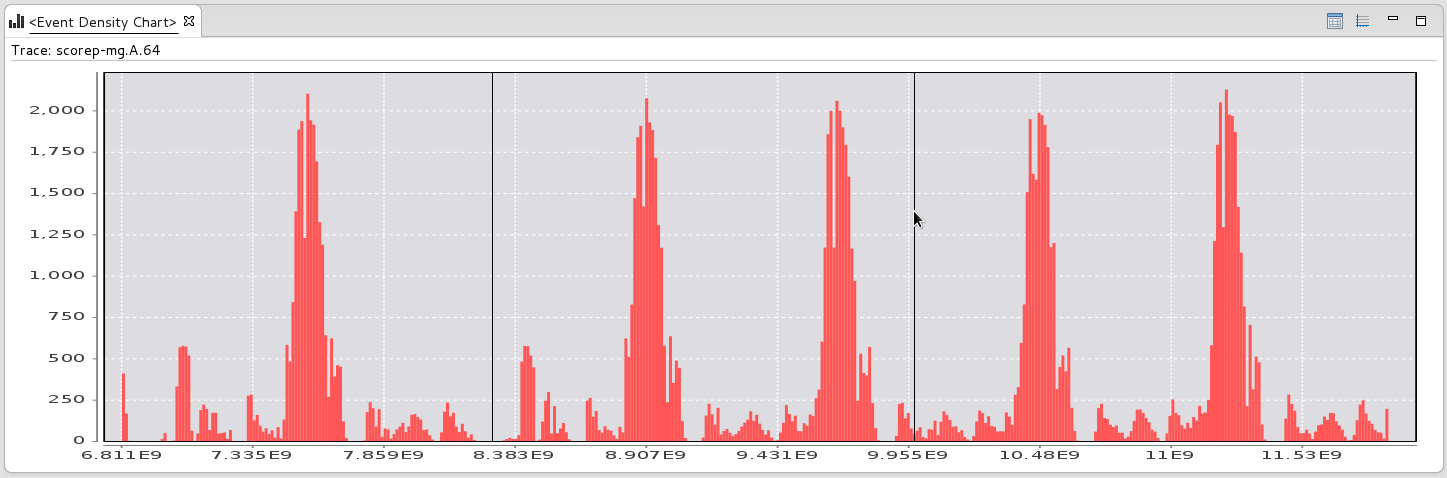
\includegraphics[width=1.0\textwidth]{images/histogram_zoom.png}
  \caption{Event Density Chart view}
  \label{fig:histogram_zoom}
\end{figure}

The \emph{Event Density Chart} view (Figure~\ref{fig:histogram_zoom}) is a Framesoc analysis view displaying the event density over time in the form of a histogram.
The $x$ axis represents the time, while the $y$ axis represents the number of events.
The histogram number of bins is fixed and has been chosen in order to ensure a clear visualization, taking into account the number of pixels actually present on a screen. 
The user can zoom and dezoom portions of the chart, using the mouse as shown in Figure~\ref{fig:histogram_zoom}.
In particular, to zoom a portion of the chart, the user has to click to the start of the portion, drag the mouse going to the right up to the end of the portion, then release the click.
To completely dezoom, the user has to do the same as above, but dragging the mouse to the left this time.
Hovering the mouse on a bin, some information about the bin is displayed (the central timestamp and the number of events).

The view toolbar contains a \emph{table} button, which triggers the visualization of the displayed portion of trace in the table view.

Note that, for the computation of the event density, all the events of the trace are considered.

%------------------------------------------------------------------
\subsection{Event Table View}
\label{subsec:table}

%%% TODO

\begin{figure}[h!]
  \centering
    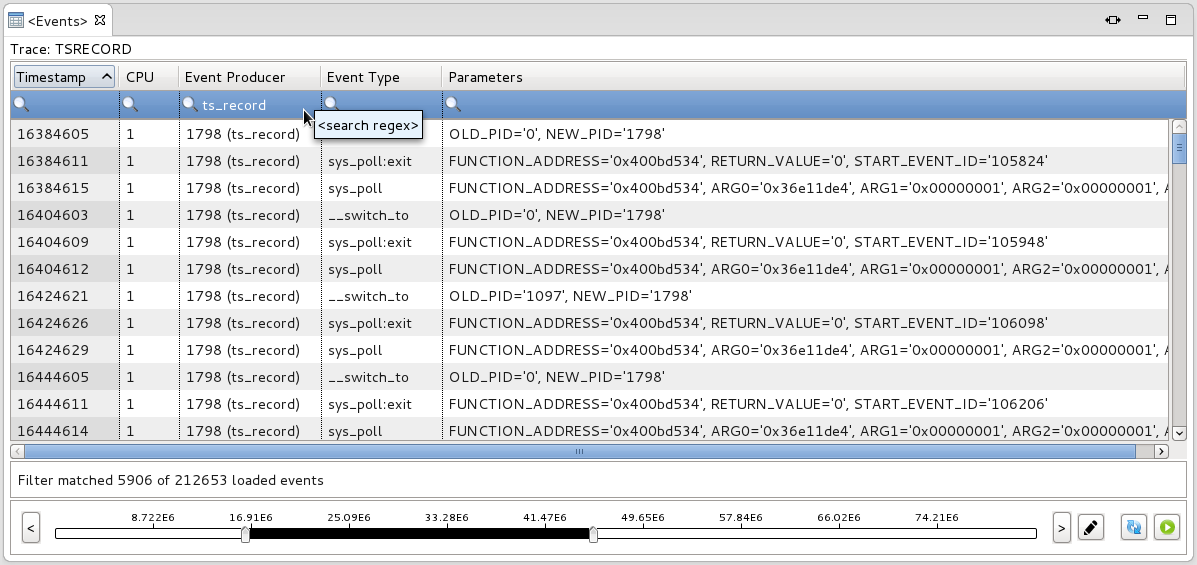
\includegraphics[width=1.0\textwidth]{images/table_nocategory.png}
  \caption{Events view}
  \label{fig:table_regex}
\end{figure}

The \emph{Events} view (Figure~\ref{fig:table_regex}) is a Framesoc analysis view showing a tabular representation of trace events.
The main element of this view is a table viewer, displaying a distinct row for each event of the trace.
This table has the following columns:
\begin{itemize}
 \item Timestamp: the event timestamp.
 \item CPU: the number of the CPU on which the event has been produced.
 \item Event Producer: the name of the entity producing the event.
 \item Event Type: the event type name.
 \item Parameters: the list of the event custom parameters, with the format NAME='VALUE'.
\end{itemize}
Each column header, when clicked, triggers the sorting of the rows according to the corresponding column. 
The first row of the table contains an editable filter for each column. 
These filters accept regular expressions.
For example, in Figure~\ref{fig:table_regex} only the events produced by a given producer are filtered.
The number of events matched by the filter, over the totality of loaded events, is shown in the status bar under the table viewer.

At the bottom of the view, there is a time management bar.
This bar contains a double range time slider (representing the whole trace duration) surrounded by two arrow buttons, and three more buttons on the right (\emph{edit}, \emph{reset} and \emph{play} buttons).
The two knobs of the double range slider identify the portion of the trace (colored in black) actually loaded in the table.
This way, the user always keeps a global visibility on the whole trace, while loading only the information he is interested in.
In order to change the time window loaded in the table, one needs to change the width of the black bar. 
However, in order to avoid spurious and useless data transfers (from disk to memory), the change is executed only when the user activates the \emph{play} button on the right of the bar.
The \emph{reset} button resynchronizes the time bar with the time window actually loaded in the table, if they differ.
In order to modify the time window visualized in the double range slider the user has several possibilities. 
\begin{itemize}
 \item Graphical selection: it is the most intuitive way and it involves using the two knobs, in order to graphically set the two bounds of the time interval.
 \item Time window navigation: this possibility involves using the two arrow buttons placed respectively on the left and on the right of the time bar, in order to select a time window that has the same size of the currently visualized one, but is located immediately before or immediately after the current one.
 \item Manual selection: by pressing the \emph{edit} button placed immediately beside the time bar on the right, the user access a dialog (Figure~\ref{fig:window_dialog}) where it is possible to explicitly put the exact values of the time interval start and end timestamps. 
 This dialog enables also a manual definition of the size of the time window to be used when performing the time window navigation described above.
\end{itemize}

\begin{figure}[h!]
  \centering
    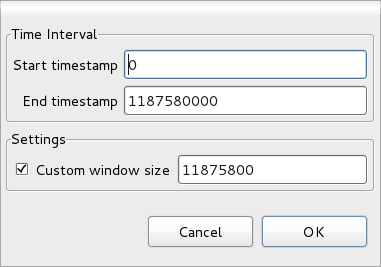
\includegraphics[width=0.35\textwidth]{images/window_dialog.png}
  \caption{Time window dialog}
  \label{fig:window_dialog}
\end{figure}

The view toolbar contains an \emph{adjust} button, which triggers column width resizing in order to fit the actual content.

%------------------------------------------------------------------
\subsection{Gantt Chart View}
\label{subsec:gantt}

%%% TODO

%------------------------------------------------------------------
\section{Framesoc Menu and Toolbar}
\label{sec:menu}

When the Framesoc perspective is activated, the Framesoc menu (Figure~\ref{fig:menu}) and the corresponding toolbar (Figure~\ref{fig:toolbar}) are visible. 

In the menu, the different functionalities are grouped in two categories: management and trace analysis.
The management menu (Figure~\ref{fig:menu_management}) allows the user to access system configuration, tool management and color management.
The trace analysis menu (Figure~\ref{fig:menu_trace_analysis}) allows the user to launch importers, analysis tools and exporter tools.

In the toolbar, the different buttons are simply shortcuts for the above functionalities, where corresponding icons mean corresponding functionalities.
The added value of the toolbar is that, beside each of the three buttons used to launch the tools of the various category (import, analysis, export), there is a drop down menu containing the list of the tools of that category, useful to directly launch a tool.

In the following subsections, the functionalities accessible from the menu or the toolbar are explained in detail.

\begin{figure}[h!]
  \centering
  \begin{subfigure}[c]{0.45\textwidth}
    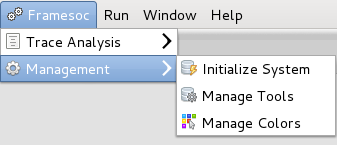
\includegraphics[width=1.0\textwidth]{images/menu_management.png}
    \caption{Management Menu}
    \label{fig:menu_management}
  \end{subfigure}
  \hspace{30pt}
  \begin{subfigure}[c]{0.45\textwidth}
    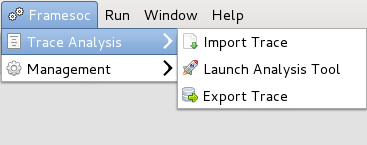
\includegraphics[width=1.0\textwidth]{images/menu_trace_analysis.png}
    \caption{Trace Analysis Menu}
    \label{fig:menu_trace_analysis}
  \end{subfigure}
  \caption{Framesoc Menu}
  \label{fig:menu}
\end{figure}

\begin{figure}[h!]
  \centering
    
\includegraphics[width=0.4\textwidth]{images/toolbar.png}
  \caption{Framesoc Toolbar}
  \label{fig:toolbar}
\end{figure}

\subsection{System Initialization}
\label{subsec:init}

At system initialization, the user accesses a configuration wizard, whose first page is shown in Figure~\ref{fig:dbms_selection}. 
This page allows the user to select the DBMS\footnote{Data Base Management System} to be used for trace storage.
In fact, as described in the technical report RT-435~\cite{pagano:hal-00830008}, Framesoc can work with several DBMS.
At the moment, the support has been implemented for SQLite (recommended) and MySQL.

\begin{figure}[h!]
  \centering
    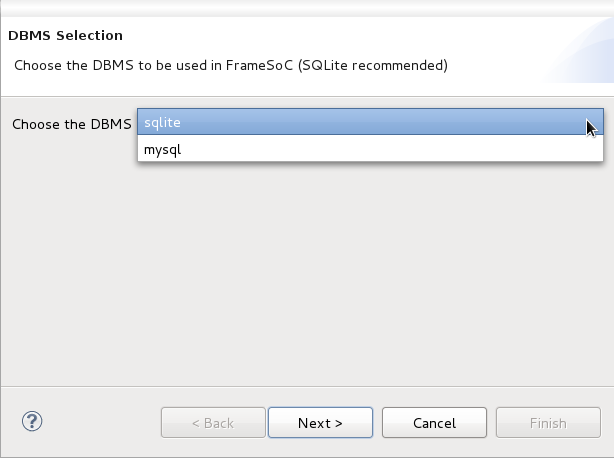
\includegraphics[width=0.5\textwidth]{images/dbms_selection.png}
  \caption{System Initialization: DBMS selection dialog}
  \label{fig:dbms_selection}
\end{figure}

Once the user has chosen the DBMS and pressed \emph{Next}, he comes to the DBMS configuration page (Figure~\ref{fig:dbms_configuration}), which is different for each DBMS.
If SQLite is selected (Figure~\ref{fig:dbms_configuration_sqlite}), the user has simply to enter the directory where he wants the database files to be kept.
Otherwise, if MySQL is chosen (Figure~\ref{fig:dbms_configuration_mysql}), the user has to specify some connection parameters (user-name, password, URL).

In both cases, after pressing \emph{Finish}, the Framesoc storage subsystem is correctly configured. 
If a System DB already exists, it is reused, otherwise a new one is created.
This configuration is saved in the Framesoc configuration file (Appendix~\ref{app:conf}). %% $\sim$/.soctrace.conf

\begin{figure}[h!]
 \centering
 \begin{subfigure}[c]{0.46\textwidth}
    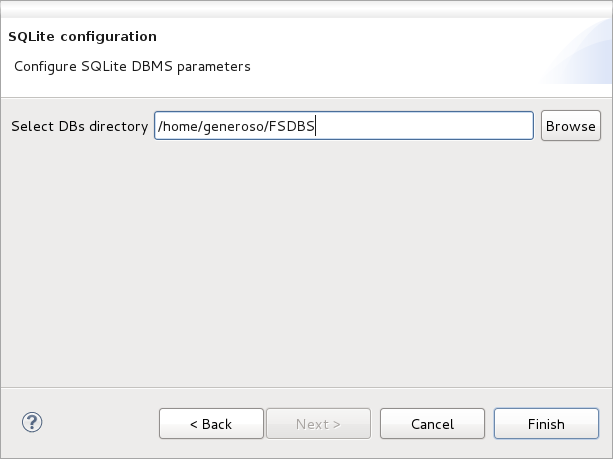
\includegraphics[width=1.0\textwidth]{images/dbms_configuration_sqlite.png}
    \caption{SQLite configuration dialog}
    \label{fig:dbms_configuration_sqlite}
 \end{subfigure}%
 \hspace{30pt}
 \begin{subfigure}[c]{0.46\textwidth}
    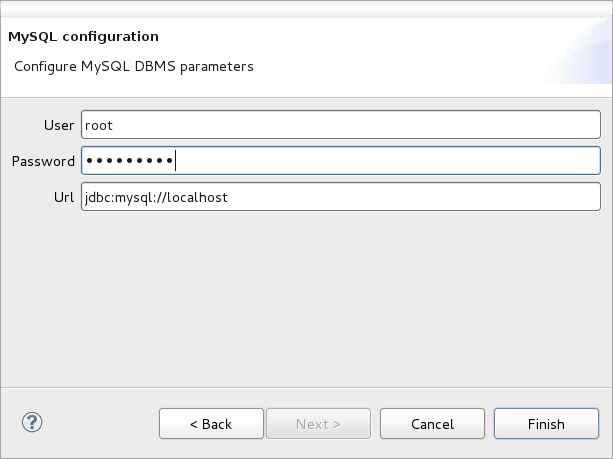
\includegraphics[width=1.0\textwidth]{images/dbms_configuration_mysql.png}
    \caption{MySQL configuration dialog}
    \label{fig:dbms_configuration_mysql}         
 \end{subfigure}
 \caption{System Initialization: DBMS configuration}
 \label{fig:dbms_configuration}       
\end{figure}

Note that after the initialization, in the case of existing System DB, if there is a mismatch between the tools registered in this System DB and the tools actually present in the Framesoc Eclipse runtime\footnote{As described in the technical report RT-435~\cite{pagano:hal-00830008} the preferred way to add tools to Framesoc is to create an Eclipse plugin, extending a specific extension point defined by Framesoc. For this reason a tool is typically a plugin in the Framesoc Eclipse runtime.}, this is automatically fixed:
\begin{itemize}
 \item If a tool exists in the DB but not in the runtime, the tool is removed with its results (if any)\footnote{The user is asked for confirmation if the \texttt{ask\_for\_tool\_removal} variable is set to \texttt{true} in Framesoc configuration file (see Appendix~\ref{app:conf})}.
 \item If a tool exists in the runtime but not in the DB, the tool is automatically registered.
\end{itemize}

Note also that at each Framesoc startup, the system automatically checks that the storage configuration is good. 
If it is not the case, the system initialization wizard is automatically launched.

A control for mismatch between runtime tools and System DB tools is equally done at each startup, with the same policy as described above.

\subsection{Tool Management}
\label{subsec:tools}

%%% TODO

The tool management dialog (Figure~\ref{fig:manage_tools}) simply displays the list of tools registered to the system, 
enabling the installation, modification and removal of external \emph{black-box} tools (tools that are not eclipse plugins).

\begin{figure}[h!]
  \centering
    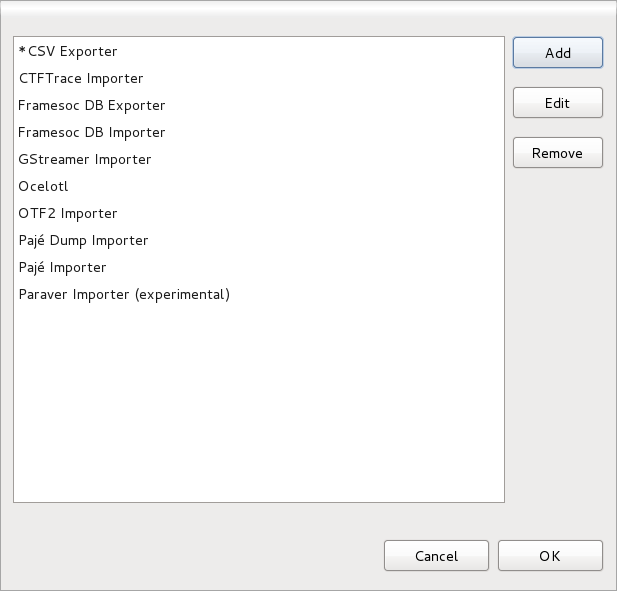
\includegraphics[width=0.5\textwidth]{images/manage_tools.png}
  \caption{Tool manager}
  \label{fig:manage_tools}
\end{figure}

\begin{figure}[h!]
  \centering
    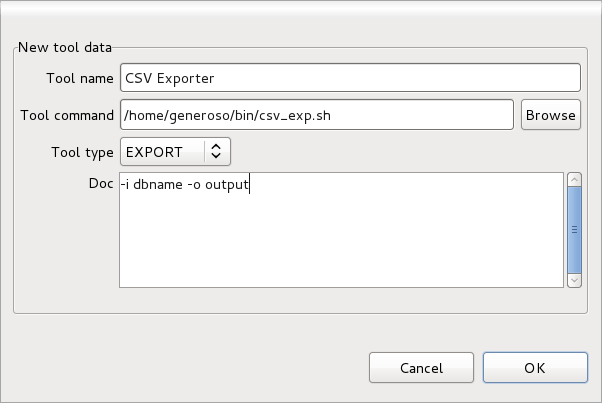
\includegraphics[width=0.5\textwidth]{images/blackbox.png}
  \caption{Black-box tool dialog}
  \label{fig:blackbox}
\end{figure}

Adding or modifying a \emph{black-box} tool requires the user to edit the different fields of the dialog displayed in Figure~\ref{fig:blackbox}.
In particular, the user has to pick a unique tool name, specify the launch command, select the tool type (import, analysis, export), write the launch documentation.

Note that the use of external \emph{black-box} tools is discouraged, since most of the functionalities available using Eclipse plugins are not available.

Note also that plugin tools cannot be added, edited or removed via the manage tool dialog, since they are managed as standard Eclipse plugins.
Plugin tools are installed and removed using the normal Eclipse procedure (\textbf{Help > Install New Software...} menu). 

\subsection{Color Management}
\label{subsec:colors}

The color management dialog (Figure~\ref{fig:color_type_list_MPI}) allows the user to modify the colors associated to event producers and event types in a centralized way for the whole workbench.
The combo box at the top of the dialog (\num{1}) enables the selection of the entity (event producer or event type).
The list below enumerates all instances for a given entity, preceded by a small square icon filled with the instance color.
The editable text field on top of this list can be used as a filter on the list.
When an entity instance is selected, pressing the \emph{edit} button (\num{2}) gives access to the color edition dialog (Figure~\ref{fig:color_editing}).
Pressing \emph{OK} saves all changes.
Pressing the \emph{reset} button (\num{3}), reverts unsaved changes.
The color configuration for a given entity is physically stored in a configuration file located in the \texttt{configuration/fr.inria.soctrace.framesoc.ui} sub-folder of the eclipse install directory.
For example, the relative path to eclipse install directory of the event type color configuration file is:
\texttt{configuration/fr.inria.soctrace.framesoc.ui/event\_type\_colors}.

\begin{figure}[h!]
  \centering
  \begin{subfigure}[c]{0.46\textwidth}
    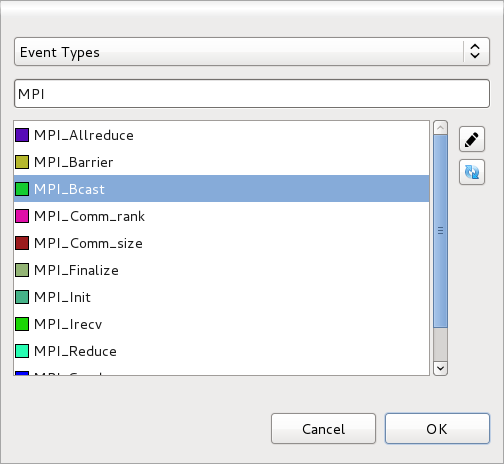
\includegraphics[width=1.0\textwidth]{images/color_type_list_MPI.png}
    \caption{Color management dialog}
    \label{fig:color_type_list_MPI}
  \end{subfigure}%
  \hspace{30pt}
  \begin{subfigure}[c]{0.46\textwidth}
    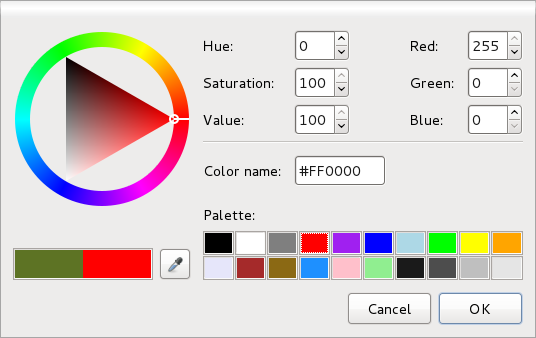
\includegraphics[width=1.0\textwidth]{images/color_editing.png}
    \caption{Color editing dialog}
    \label{fig:color_editing}       
  \end{subfigure}%
  \caption{Framesoc Color Management}
  \label{fig:colors}       
 \end{figure}

Note that when \emph{OK} is pressed after changing some colors, the workbench modules are notified and the views may react by updating their colors in real-time.

\subsection{Trace Import}
\label{subsec:import}

The trace import dialog (Figure~\ref{fig:import_dialog}) allows the user to import a new trace into the system using one of the registered importer tools.
The user selects the importer from the combo box at the top, then he specifies the trace files (if more than one file is needed, all the files should be selected in the browser dialog opened when the \emph{Browse} button is pressed). 
If the importer requires additional parameters (the \emph{Doc} field normally provides this information), the user specifies these parameters too.
At the botton of the dialog, there is an \emph{Error Message} zone, intended to inform the user about any error in the input.

Finally, after pressing \emph{OK}, the import process is launched with the provided input.
At the end of this process, the trace browser view is automatically updated with the new trace information.

\begin{figure}[h!]
  \centering
    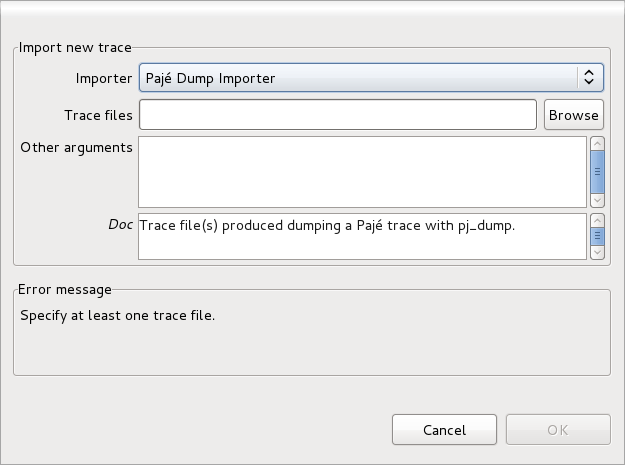
\includegraphics[width=0.5\textwidth]{images/import_dialog.png}
  \caption{Import trace dialog}
  \label{fig:import_dialog}
\end{figure}

\subsection{Launch Analysis Tool}
\label{subsec:analysis}

The launch analysis tool dialog (Figure~\ref{fig:analysis_dialog}) allows the user to launch one of the analysis tools registered to the system.
The user selects the analysis tool from the combo box at the top. 
If the tool requires additional parameters (the \emph{Doc} field normally provides this information), the user specifies these parameters too. 
At the botton of the dialog, there is an \emph{Error Message} zone, intended to inform the user about any error in the input.
Finally, after pressing \emph{OK}, the tool is launched with the provided input. 

\begin{figure}[h!]
  \centering
    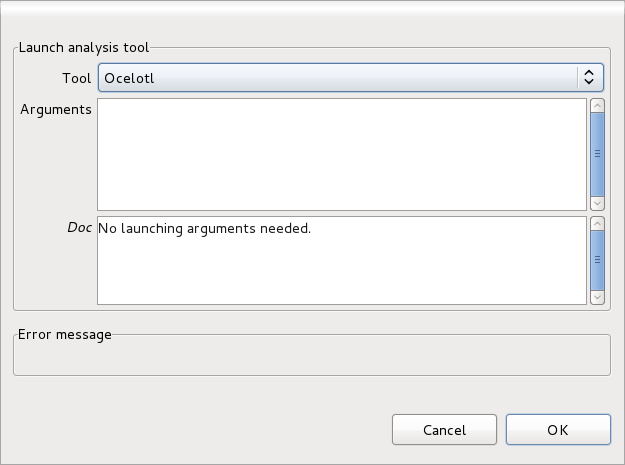
\includegraphics[width=0.5\textwidth]{images/analysis_dialog.png}
  \caption{Launch analysis dialog}
  \label{fig:analysis_dialog}
\end{figure}

\subsection{Trace Export }
\label{subsec:export}

The  trace export dialog (Figure~\ref{fig:export_dialog}) works exactly as the launch analysis tool dialog, with the difference that this time the user can launch one of the exporter tools registered to the system.

\begin{figure}[h!]
  \centering
    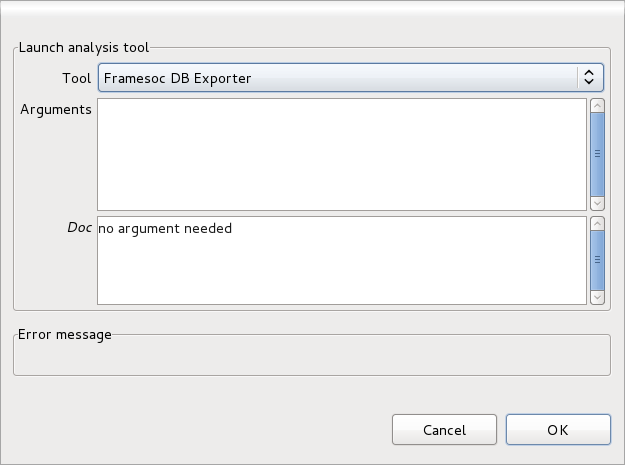
\includegraphics[width=0.5\textwidth]{images/export_dialog.png}
  \caption{Export trace dialog}
  \label{fig:export_dialog}
\end{figure}

\newpage

\appendix

%%=====================================================================
\section{Framesoc Configuration File}
\label{app:conf}
%%=====================================================================

The Framesoc configuration file (\texttt{.soctrace.conf}) is located in the user home directory.
It is automatically generated and mostly configurable using the GUI.

The file contains the following parameters:
\begin{description}
 \item[soctrace\_dbms]: DBMS used by Framesoc. The accepted values are: sqlite, mysql.
 \item[mysql\_db\_user]: MySQL database user name.
 \item[mysql\_db\_password]: MySQL database user name.
 \item[mysql\_base\_db\_jdbc\_url]: MySQL database connection URL.
 \item[sqlite\_db\_directory]: Directory containing the SQLite database files.
 \item[soctrace\_db\_name]: Name of the Framesoc System DB.
 \item[max\_view\_instances]: Maximum number of instances for a given type of analysis views.
 \item[trace\_db\_indexing]: Boolean stating if automatic time indexing is done at trace import.
 \item[ask\_for\_tool\_removal]: Boolean stating if user confirmation must be asked when removing a tool and its results.
\end{description}

%% bibliography
\newpage
\renewcommand{\refname}{References}
\bibliography{framesoc_biblio}{}
\bibliographystyle{unsrt}
%%

%%=====================================================================
%%=====================================================================
\end{sloppypar} 
\end{document}
%%=====================================================================
%%=====================================================================

\endinput
%%
%% End of file.
